\documentclass{beamer}
\usepackage[utf8]{inputenc}
\usepackage[francais]{babel}
\usepackage{amsmath}
\usepackage[squaren,Gray]{SIunits}
\usepackage{numprint}
\usepackage{amsfonts}
\usepackage{amssymb}
\usepackage{graphicx}
\usepackage{mathtools}
\usepackage{mhchem}
\usepackage{hyperref}
\usepackage{varwidth}
\usetheme{Warsaw}
\title{Présentation Tâche 2:\\ création d’un flow-sheet plus détaillé et analyse paramétrique 

}
\author{Groupe 1246}
\institute{École Polytechnique de Louvain}
\date{}
\begin{document}

\begin{frame}
\titlepage
\end{frame}


\begin{frame}
\frametitle{La dernière étape du procédé}
\framesubtitle{avec un exemple de sous-titre}

Le procédé \textsc{Haber-Bosch}

$$\ce{N_2} + \ce{3H_2} \xrightleftharpoons[\mathit{endo}]{\mathit{exo}} \ce{2NH_3}$$

Supposition avec le principe de \textsc{Le Chatelier}: quand la température diminue, le rendement augmente. 

\end{frame}




\begin{frame}
\frametitle{Analyse paramétrique avec \textsc{Matlab}}
\framesubtitle{avec un exemple de sous-titre}

\begin{empheq}[left=\empheqlbrace]{align}
& F_{mol,\ce{Ar}_{in}}  + \mu \frac{ X - \mu (X-\xi)}{78(1-\mu)} = \frac{ X - \mu (X-\xi)}{78(1-\mu)} \\
& F_{mol,\ce{N2}_{in}} + \mu (X-\xi) = X \\
& F_{mol,\ce{H2}_{in}}  + \mu (3X - 3\xi) = 3X \\
& K(T) = \left( \dfrac{4 \xi^2 \cdot (4X - 2\xi + \frac{ X - \mu (X-\xi)}{78(1-\mu)})^2}{(3X-3\xi)^3 \cdot (X-\xi) \cdot p^2}\right) 
\end{empheq}

\end{frame}



\begin{frame}
\frametitle{Analyse paramétrique avec \textsc{Matlab}}
\framesubtitle{avec un exemple de sous-titre}

\begin{figure}[ht!]
\centering
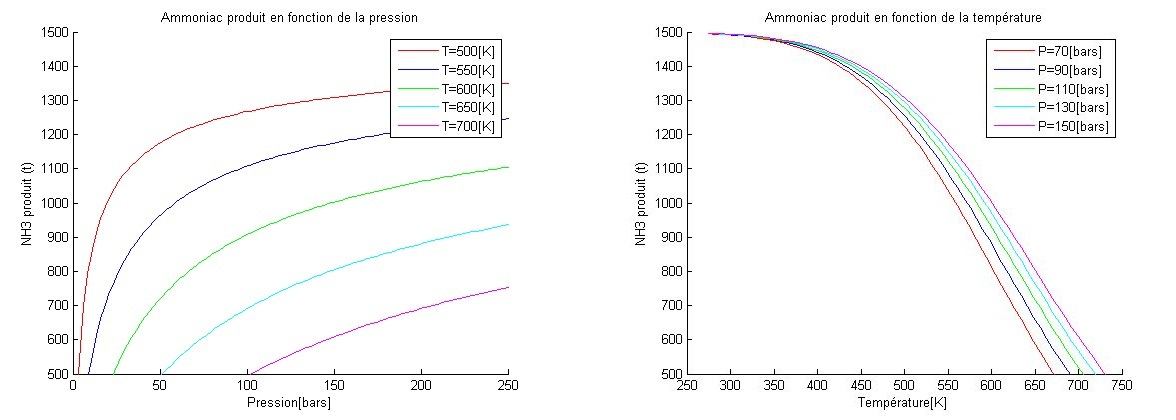
\includegraphics[scale=0.2]{fct_pression.jpg}
\end{figure}


\end{frame}


\end{document}
